\section{Análise das Simulações}

\subsection{Cenário 1}
O cenário 1 foi o primeiro a ser desenvolvido e o mais básico, a intenção foi
incrementar outras variáveis com o desenvolvimento de outros cenários e como o cenário
1 foi o menos complexo pode ser feita diversas análises tendo como a principal, uma
modelagem matemática do cenário. Para termos noção das simulações e um bom
equilíbrio dos resultados, foi considerado por padrão de valores fixos do cenário os
seguintes: tamanho fixo de 50 bases, 500 moléculas iniciais, 20\% eficiência de filtro
(chance de uma moléculas não-afim morrer), 0\% de chance de uma molécula afim morrer,
5\% de taxa de mutação, 500 moléculas de totais no round e o tamanho do filtro era de 5
bases onde a sequência era escolhida aleatoriamente no início.

\subsubsection{Variando a taxa de mutação}

\begin{figure}[!h]
    \centering
    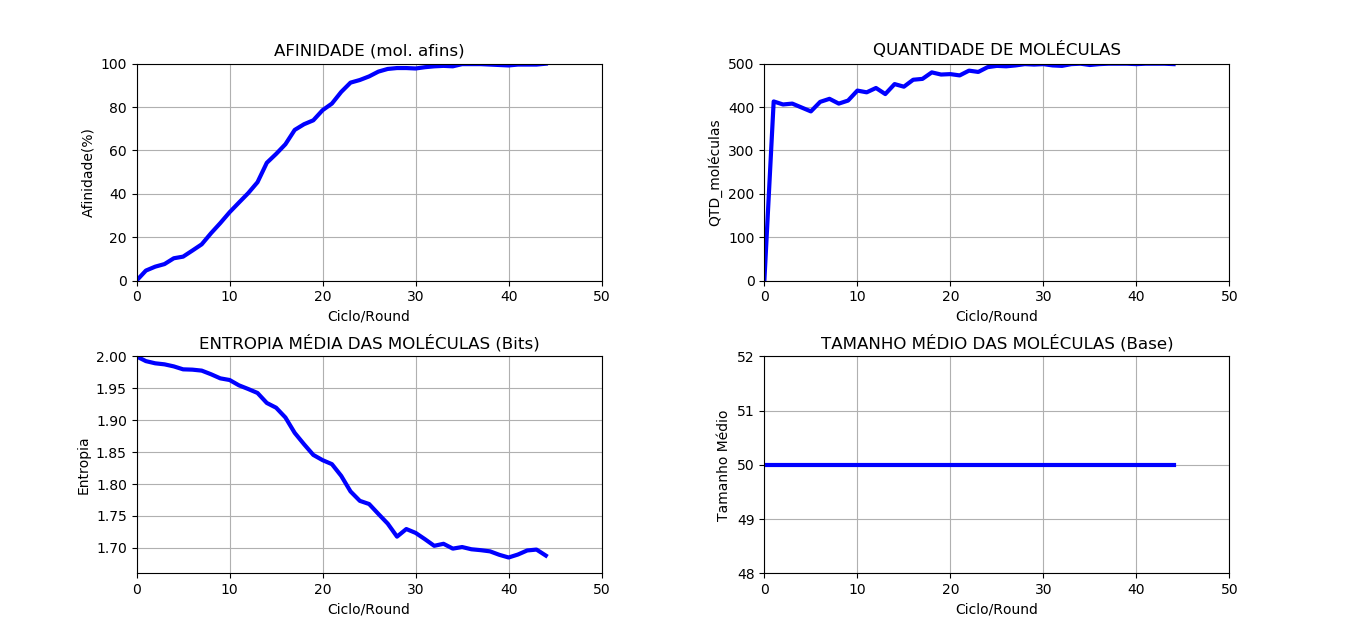
\includegraphics[width=15cm]{figures/image1_alpha00_beta_20.png}
    \caption{Cenário 1- Taxa de mutação 0\%.}
    \label{fig:image1_alpha00_beta_20}
\end{figure}

\begin{figure}[!h]
    \centering
    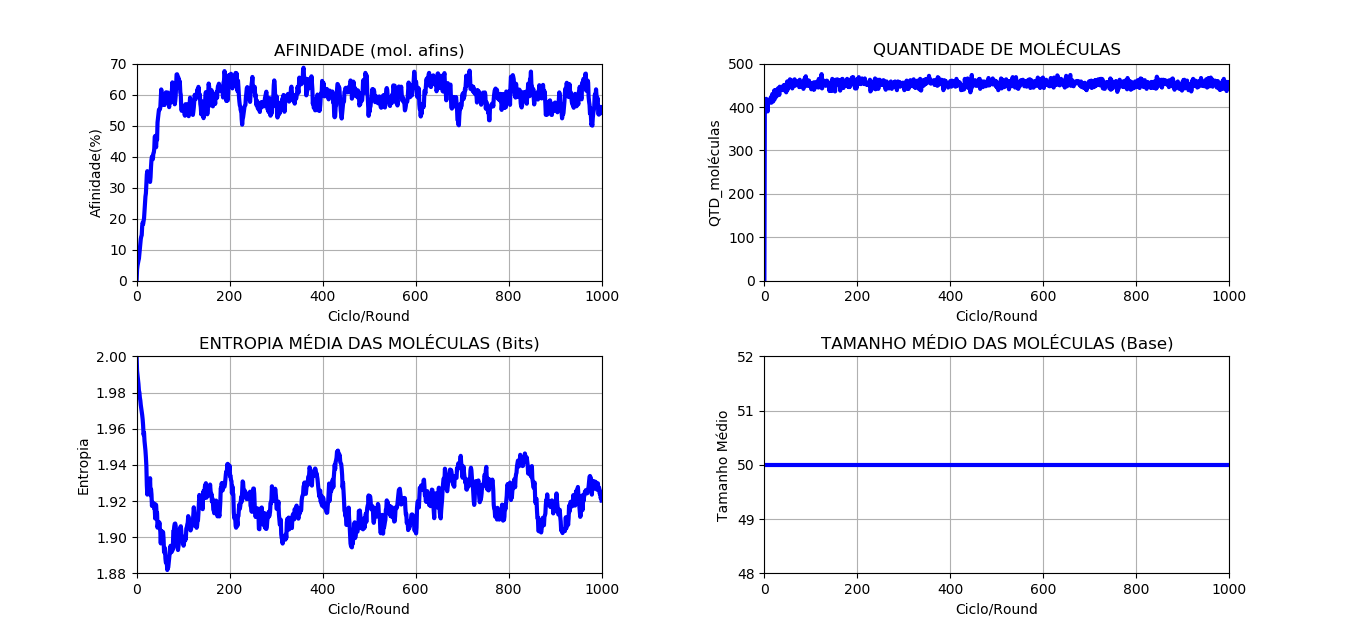
\includegraphics[width=15cm]{figures/image2_alpha05_beta_20.png}
    \caption{Cenário 1- Taxa de mutação 5\%.}
    \label{fig:image2_alpha05_beta_20}
\end{figure}

\begin{figure}[!h]
    \centering
    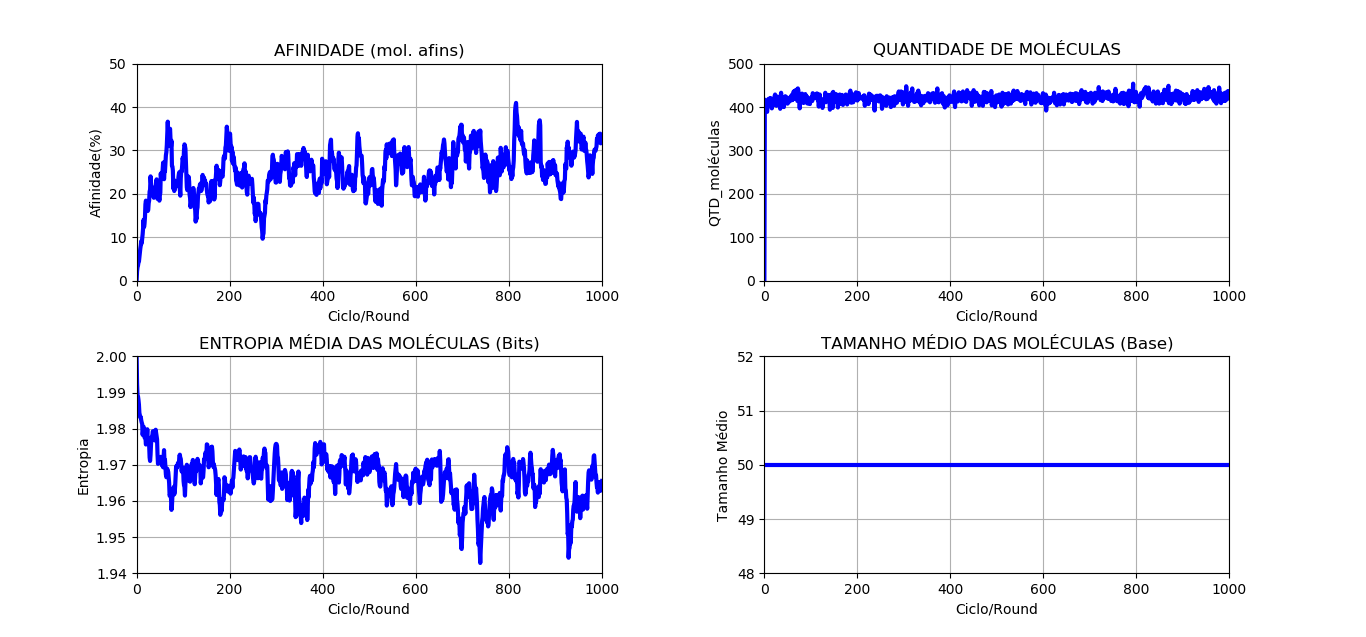
\includegraphics[width=15cm]{figures/image3_alpha10_beta_20.png}
    \caption{Cenário 1- Taxa de mutação 10\%.}
    \label{fig:image3_alpha10_beta_20}
\end{figure}


\begin{figure}[!h]
    \centering
    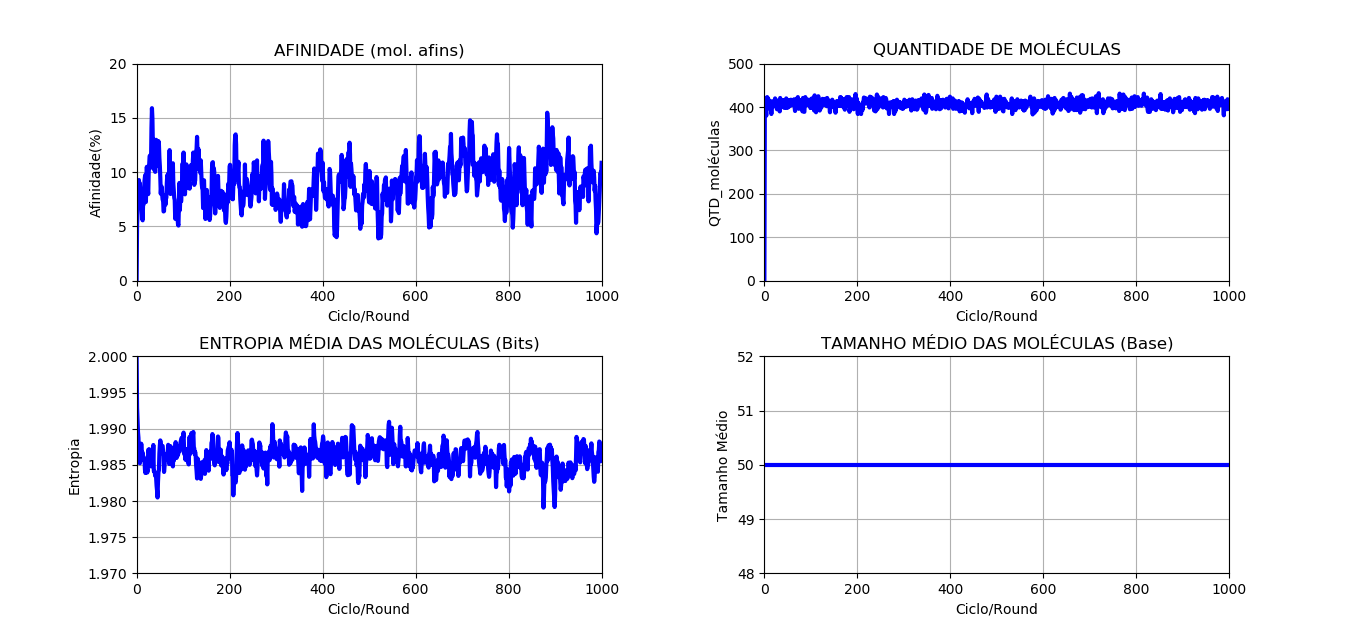
\includegraphics[width=15cm]{figures/image4_alpha20_beta_20.png}
    \caption{Cenário 1- Taxa de mutação 20\%.}
    \label{fig:image4_alpha20_beta_20}
\end{figure}

\begin{figure}[!h]
    \centering
    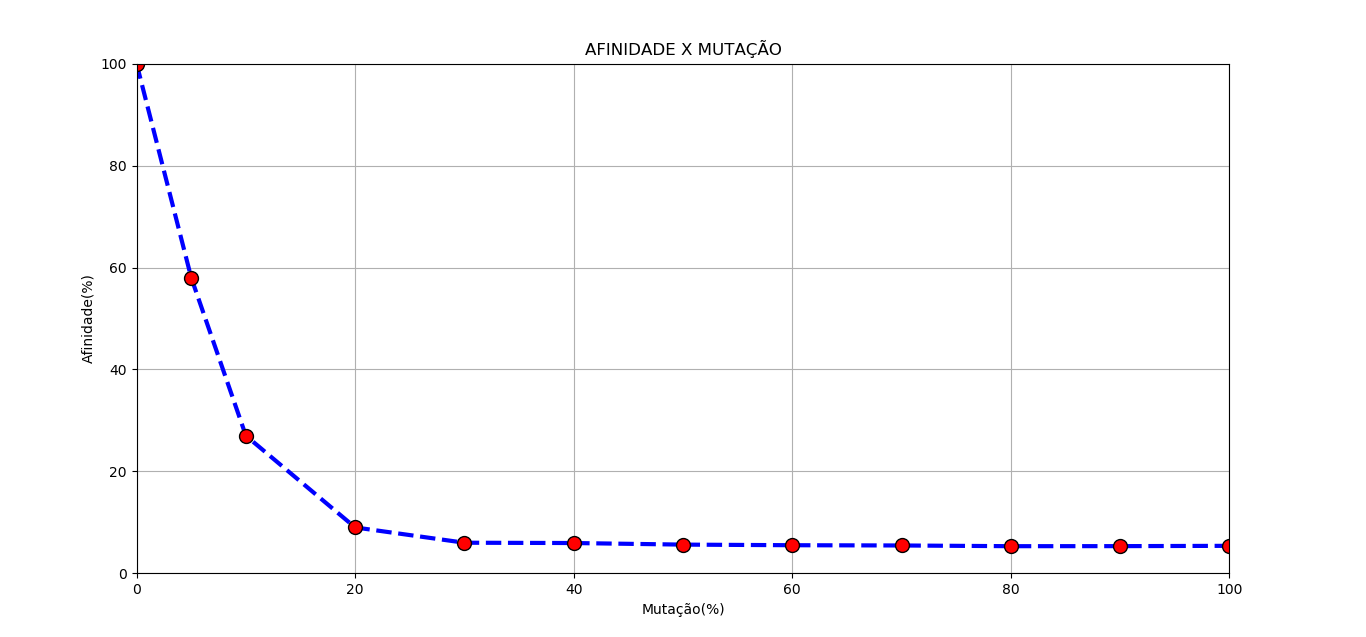
\includegraphics[width=15cm]{figures/affinity_mutation.png}
    \caption{Relação entre afinidade e taxa de mutação.}
    \label{fig:affinity_mutation}
\end{figure}

\newpage
Como pode-se reparar, ao observar as figuras \ref{fig:image1_alpha00_beta_20}-\ref{fig:image4_alpha20_beta_20} podemos perceber que o único momento em que a afinidade bate 100\% a simulação tem 0\% de mutação e que com
somente 5\% de mutação, a afinidade fica em média de 60\% mostrando que a porcentagem
de afinidade é muito sensível a mutação. Na figura \ref{fig:affinity_mutation} temos uma referência que a partir
de 20\% de mutação a afinidade fica menor que 10\% se tornando mínima a quantidade de
moléculas aptas ao filtro.

\subsubsection{Variando a eficiência do filtro}

\begin{figure}[!h]
    \centering
    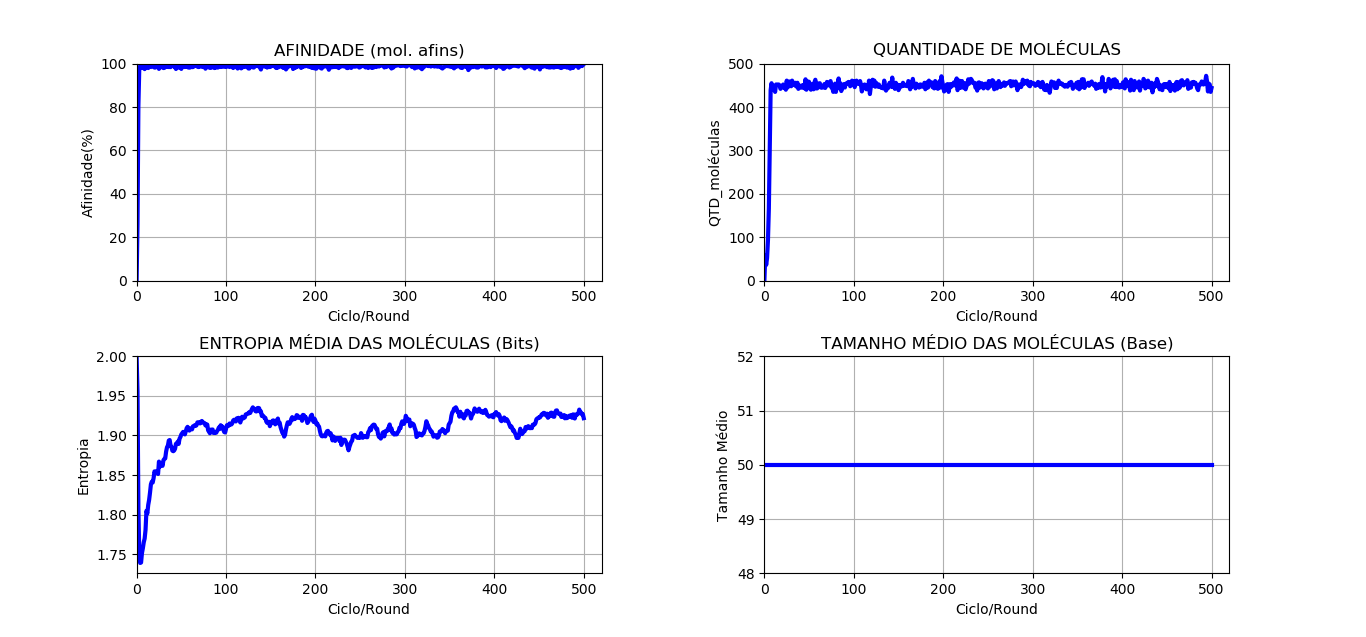
\includegraphics[width=15cm]{figures/image9_alpha05_beta_90.png}
    \caption{Eficiência de filtro 90\%.}
    \label{fig:image9_alpha05_beta_90}
\end{figure}

\begin{figure}[!h]
    \centering
    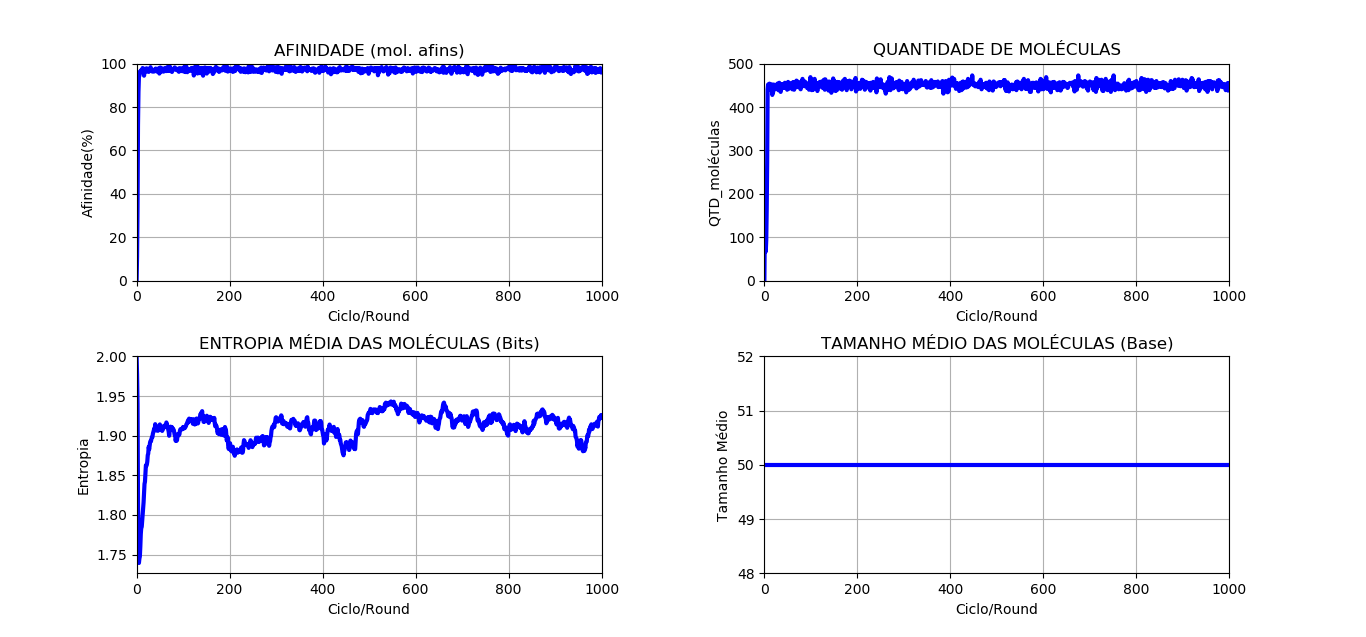
\includegraphics[width=15cm]{figures/image8_alpha05_beta_80.png}
    \caption{Eficiência de filtro 80\%.}
    \label{fig:image8_alpha05_beta_80}
\end{figure}

\begin{figure}[!h]
    \centering
    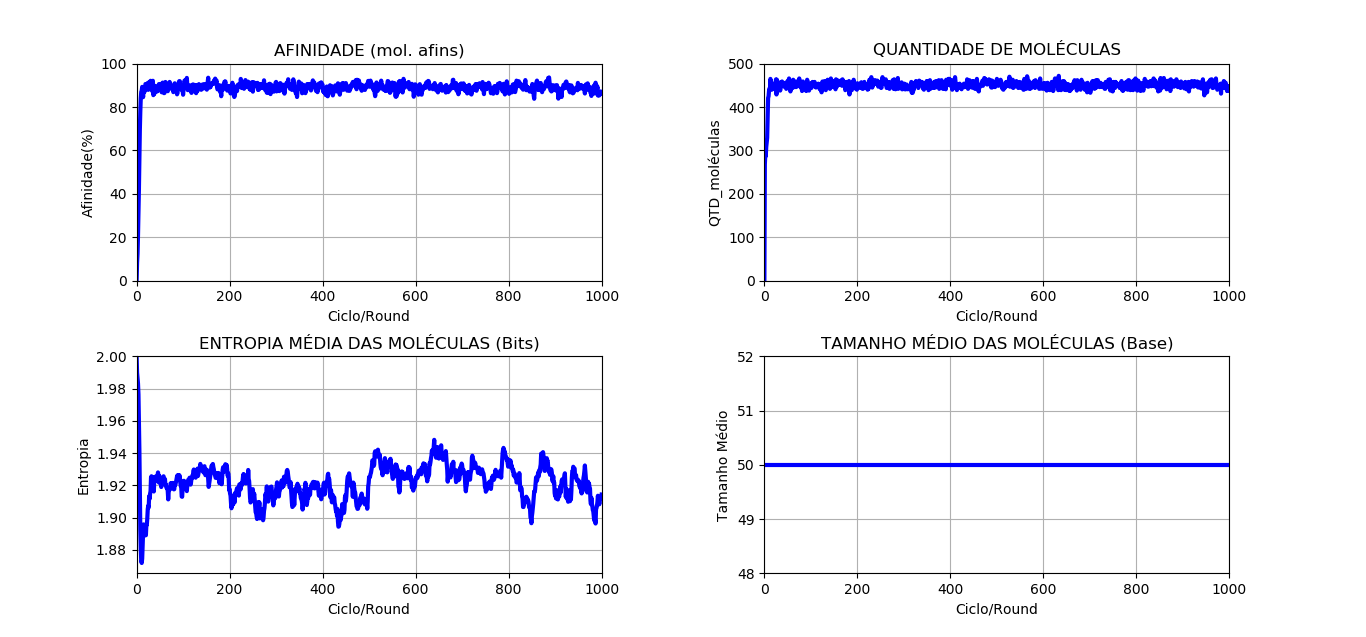
\includegraphics[width=15cm]{figures/image7_alpha05_beta_50.png}
    \caption{Eficiência de filtro 50\%.}
    \label{fig:image7_alpha05_beta_50}
\end{figure}

\begin{figure}[!h]
    \centering
    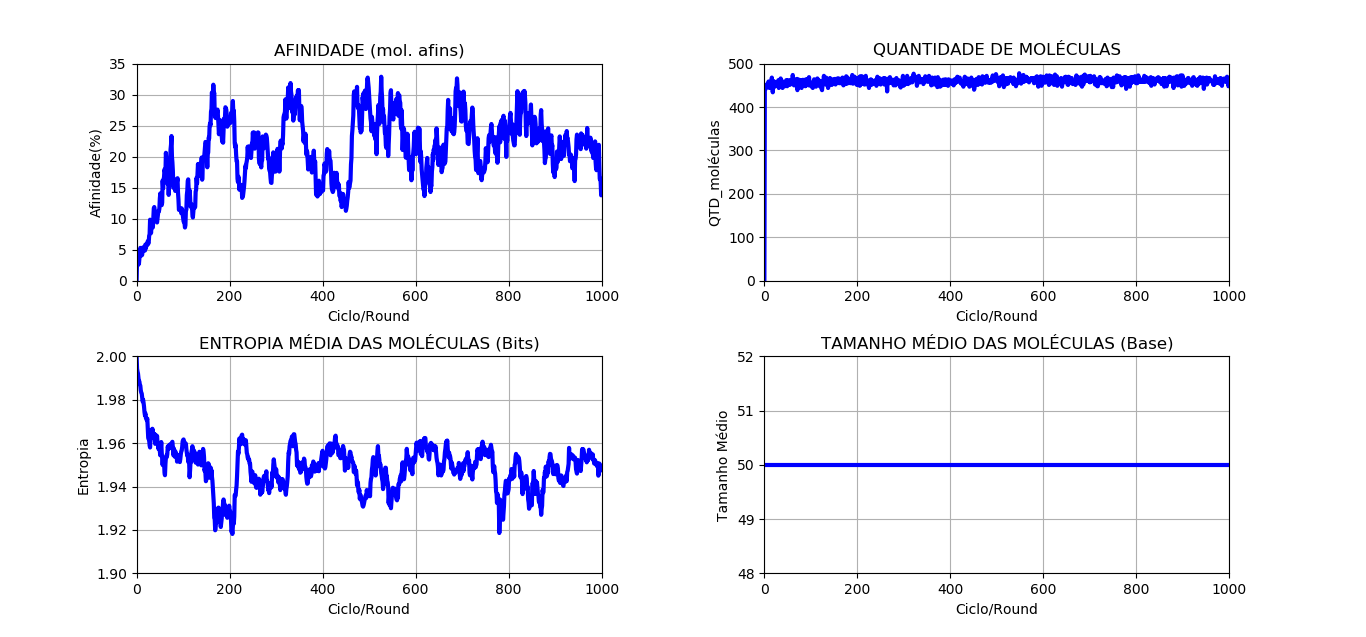
\includegraphics[width=15cm]{figures/image6_alpha05_beta_10.png}
    \caption{Eficiência de filtro 10\%.}
    \label{fig:image6_alpha05_beta_10}
\end{figure}

\begin{figure}[!h]
    \centering
    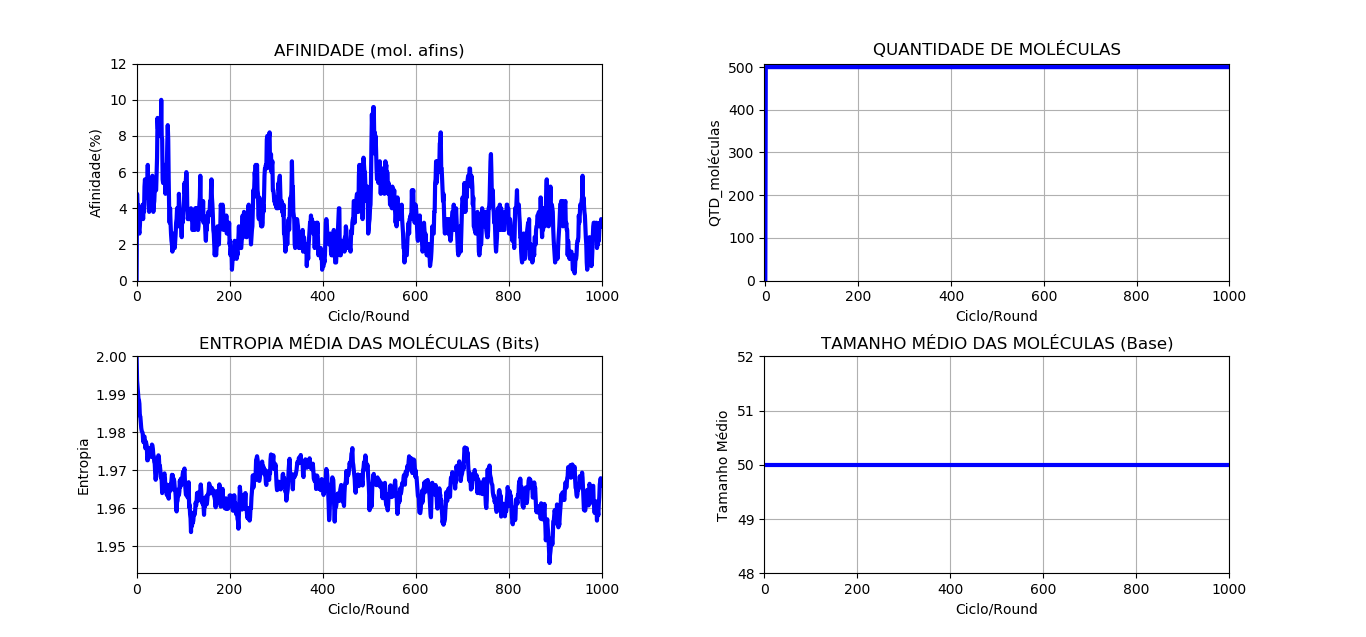
\includegraphics[width=15cm]{figures/image5_alpha05_beta_00.png}
    \caption{Eficiência de filtro 0\%.}
    \label{fig:image5_alpha05_beta_0}
\end{figure}

\begin{figure}[!h]
    \centering
    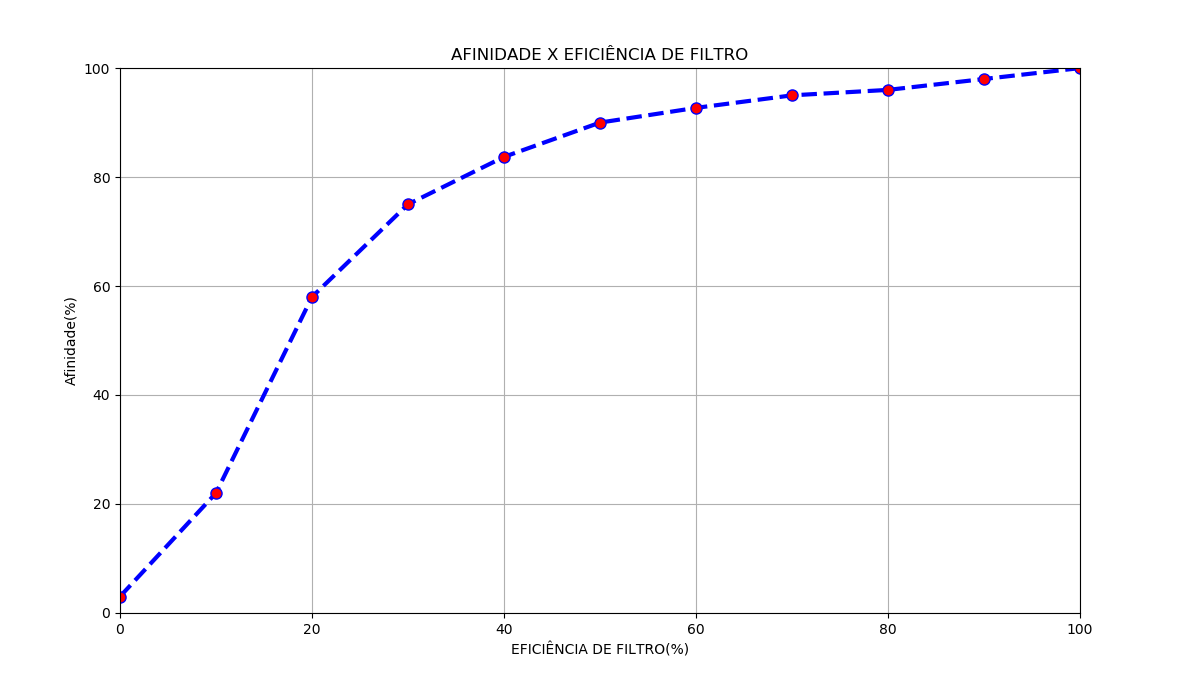
\includegraphics[width=15cm]{figures/affinity_filter.png}
    \caption{Relação entre afinidade e eficiência de filtro.}
    \label{fig:affinity_filter}
\end{figure}

\newpage
Com bases nas figuras \ref{fig:image9_alpha05_beta_90}-\ref{fig:image5_alpha05_beta_0}, pode-se perceber que a afinidade se decai muito
quando é menor que 20\% de eficiência de filtro, acima desse valor tanto a afinidade
quanto a quantidade de moléculas não são tão sensíveis caso tenha uma mudança mínima
de eficiência. Qualquer valor acima de 20\% seria um bom valor para a simulação. 

\subsubsection{Presença de 2 filtros}

\begin{figure}[!h]
    \centering
    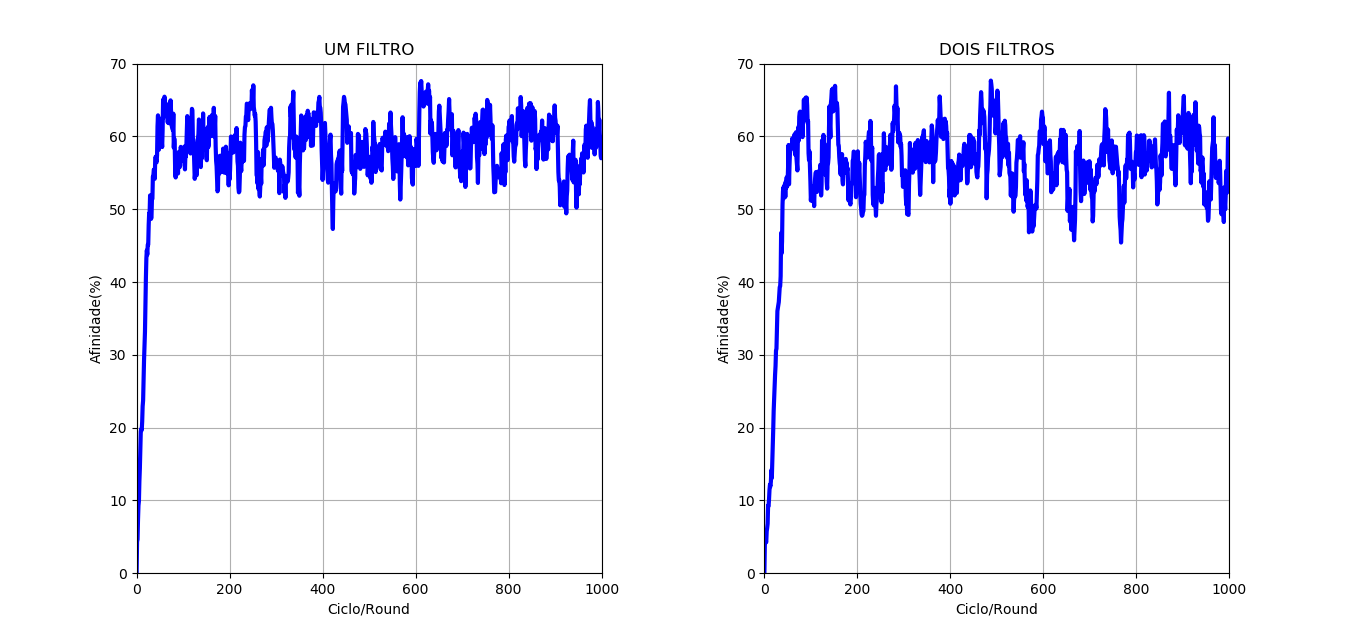
\includegraphics[width=15cm]{figures/image14_alpha05_beta_1de20_e_2de10.png}
    \caption{Comparação entre 1 filtro de 20\%  e 2 filtros de 10\%}
    \label{fig:image14_alpha05_beta_1de20_e_2de10}
\end{figure}
\newpage

A intenção dessa simulação foi mostrar que não tem tanta diferença em
acrescentar mais filtros se eles forem iguais (buscarem a mesma sequência) pois basta
aumentar a força do filtro que você tem em mãos, na figura \ref{fig:image14_alpha05_beta_1de20_e_2de10} pode-se perceber que os valores são idênticos. 

\subsubsection{Equação modelada}

\begin{equation}
    Q(t) = ( 1 - diff_i )[N_A + (1 - \alpha )N_A + N_B + 2N_B + \alfa N_A]
\end{equation}
Onde:
\begin{equation}
    diff = \left\{\begin{matrix}
        0
        &\hbox{, se popMax }\geq Q_{t + \frac{1}{2}}\\ 
        \frac{Q_{t + \frac{1}{2} - popMax}}{Q_{t + \frac{1}{2}}}
        &\hbox{, se popMax }< Q_{t + \frac{1}{2}}
    \end{matrix}\right.
\end{equation}
e
\begin{equation}
    Q_{t + \frac{1}{2}\ =\ 2(N_A + N_B)}
\end{equation}

\vspace{1cm}

\begin{flushleft}
\begin{tabular}{l|l}
Q(t)     & Quantidade de moléculas no tempo “t” (ciclo ou round) \\
$\alpha$ & Taxa de mutação\\
$\beta$  &Taxa de eficiência de filtro\\
$N_A$       & Quantidade de moléculas afins\\
$N_B$       & Quantidade de moléculas não-afins\\
Diff        & Corte na quantidade de moléculas\\
\end{tabular}
\end{flushleft}

\begin{figure}[!h]
    \centering
    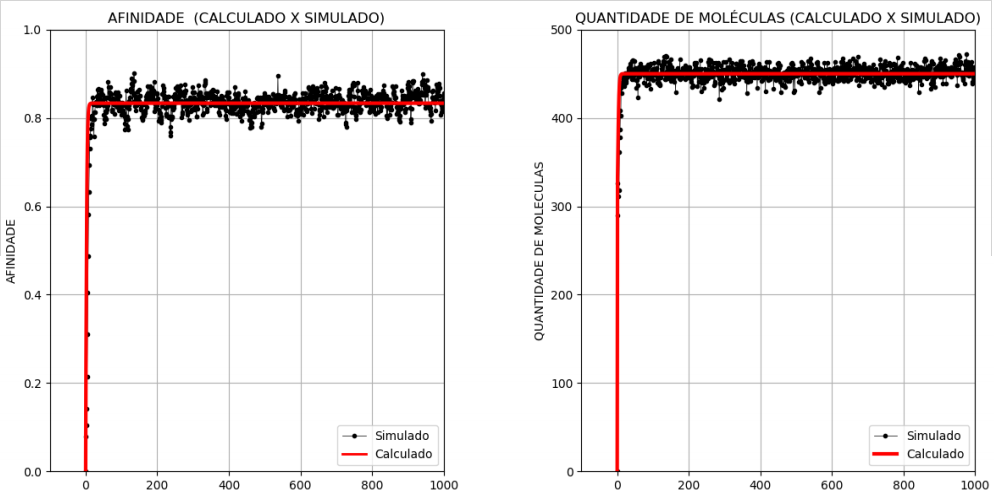
\includegraphics[width=15cm,height=6cm]{figures/img-calculated-simulated.png}
    \caption{Cenário 1- Comparando método Simulado com Calculado.}
    \label{fig:img-calculated-simulated}
\end{figure}
\newpage

Esse foi sem dúvidas o melhor resultado dos cenários, tanto a afinidade quanto a
quantidade de moléculas são bem parecidas, foi testado com a eficiência de filtro 40\% e
variando a mutação entre 5\%, 10\%, 15\% e 20\%. Na figura 15 é referente a 5\% de taxa de
mutação. A equação 5 se refere a ação do ciclo onde temos sua replicação, já na equação
4 representa o fator de diminuição, caso as moléculas passem de 500 elas são cortadas até
o seu limite. Na equação 3 é modelada com bases nos passos do método simulado.

\subsection{Cenário 2}

O cenário 2 teve incremento de duas novas variáveis, quebra e junção. A intenção é
analisar o quão diferente vai ser essa mudança entre o cenário 1 e 2, como vai ser o
comportamento do tamanho das moléculas e a afinidade e quantidade perante essas
modificações. Novamente, para termos noção das simulações e um bom equilíbrio dos
resultados, foi considerado por padrão de valores fixos do cenário os seguintes: tamanho
inicial de 50 bases, 500 moléculas iniciais, 20\% eficiência de filtro (chance de uma
moléculas não-afim morrer), 0\% de chance de uma molécula afim morrer, 5\% de taxa de
mutação, 500 moléculas de totais no round e o tamanho do filtro era de 5 bases onde a
sequência era escolhida aleatoriamente no início. Quanto aos valores de quebra e junção
foram: 100\% de chance de uma molécula se quebrar caso encontre a sequência de 3 bases
escolhida \emph{TTT} o stop códon, já o processo de junção, foram escolhidas as 5 bases
complementares da sequência escolhida pelo filtro para uma molécula ser apta (se a
sequência afim fosse AATTG seu complemento seria TTAAC) com 100\% de chance de junção.

\subsubsection{Variando a taxa de mutação}

\begin{figure}[!h]
    \centering
    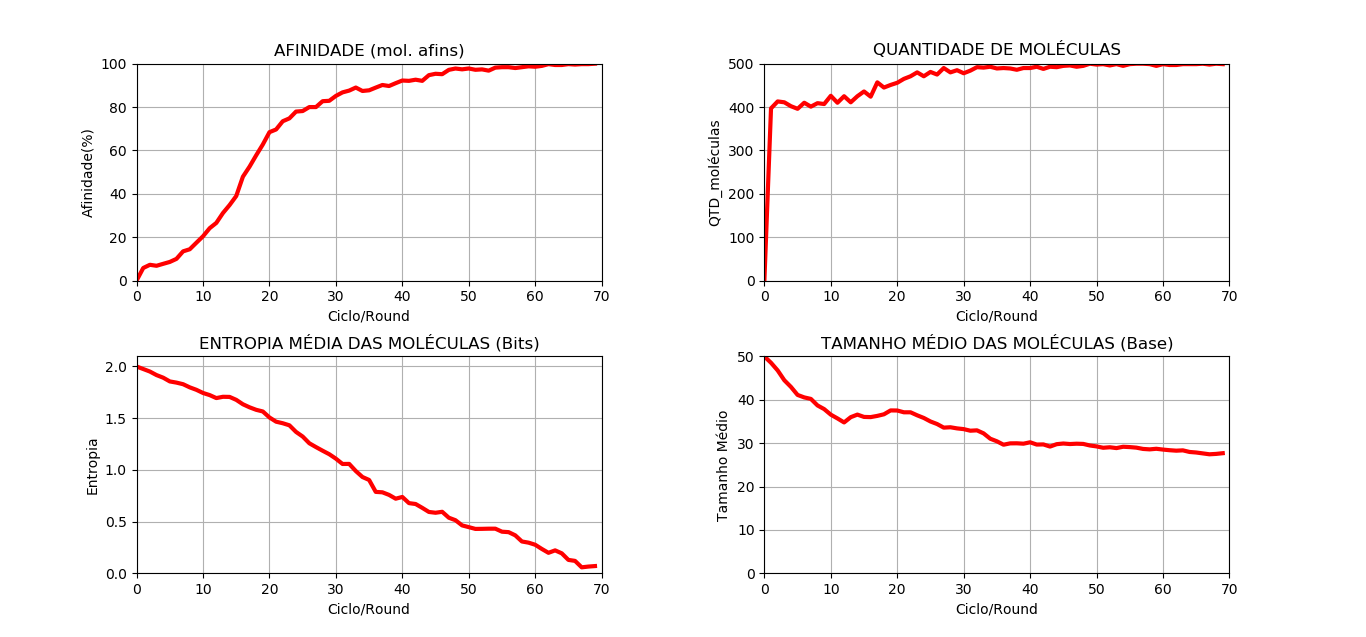
\includegraphics[width=15cm,height=7cm]{figures/image15_alpha00_beta_20.png}
    \caption{Cenário 2- Taxa de mutação 0\%.}
    \label{fig:image15_alpha00_beta_20}
\end{figure}

\begin{figure}[!h]
    \centering
    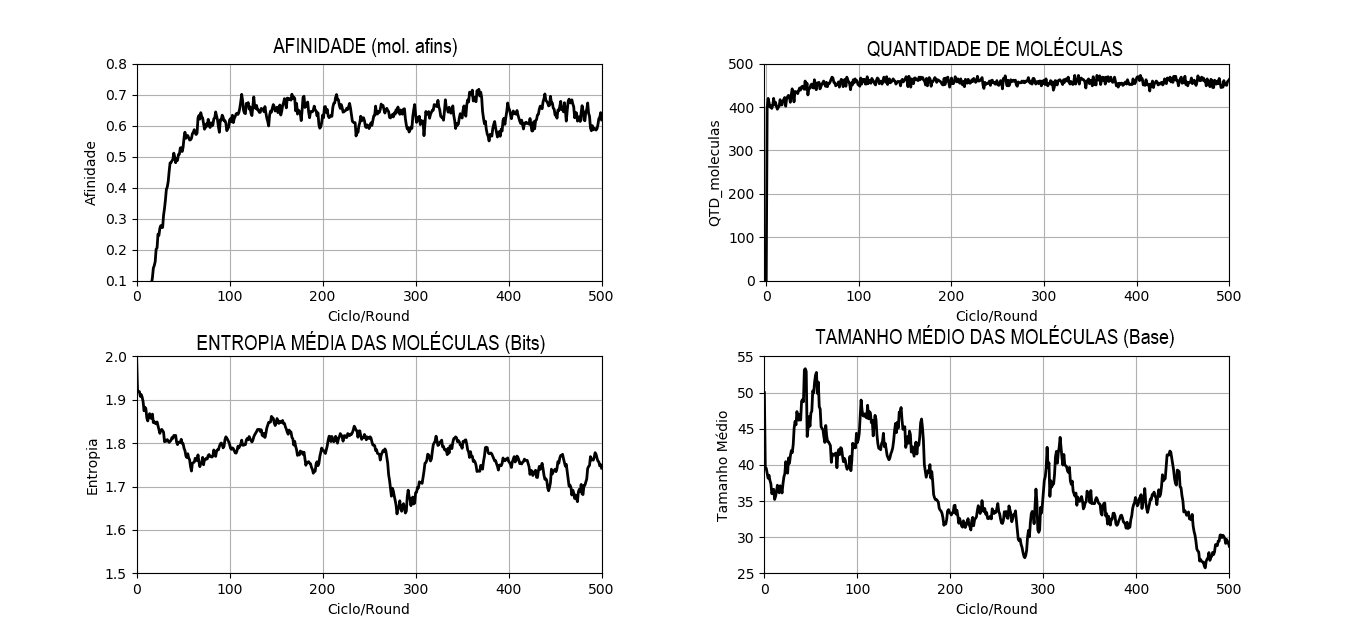
\includegraphics[width=15cm,height=7cm]{figures/image16_alpha05_beta_20.png}
    \caption{Cenário 2 - Taxa de mutação 5\%.}
    \label{fig:image16_alpha05_beta_20}
\end{figure}

\begin{figure}[!h]
    \centering
    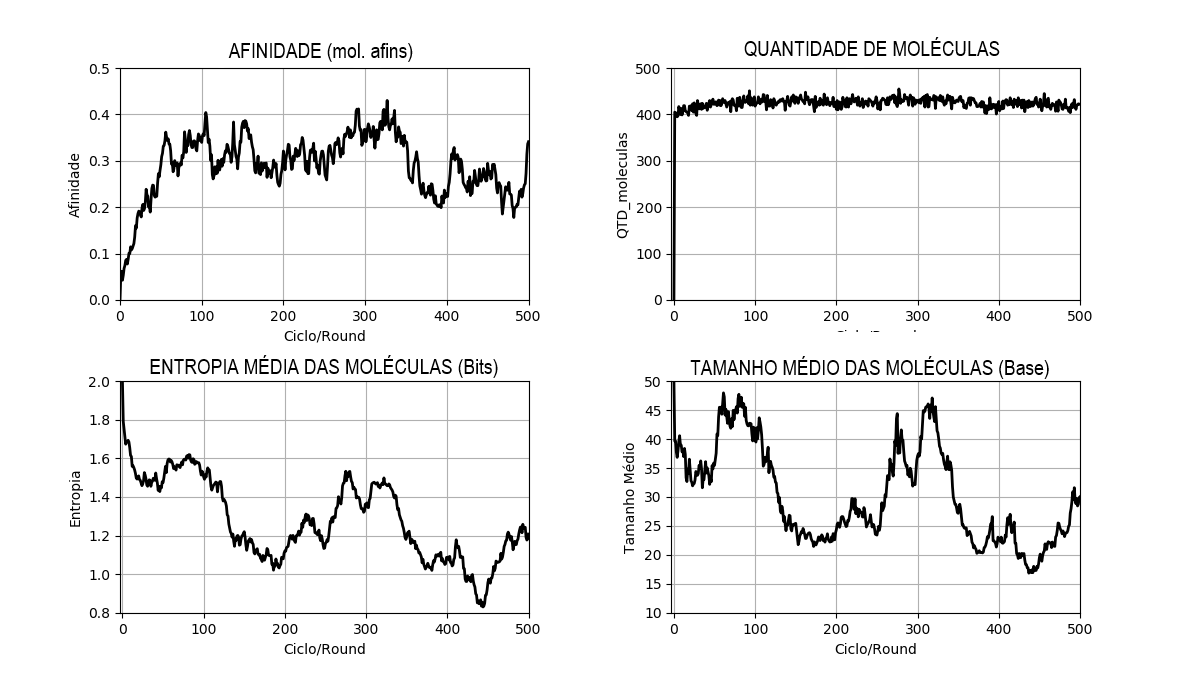
\includegraphics[width=15cm,height=7cm]{figures/image17_alpha10_beta_20.png}
    \caption{Cenário 2 - Taxa de mutação 10\%.}
    \label{fig:image17_alpha10_beta_20}
\end{figure}

\newpage

\subsubsection{Variando a eficiência do filtro}

\begin{figure}[!h]
    \centering
    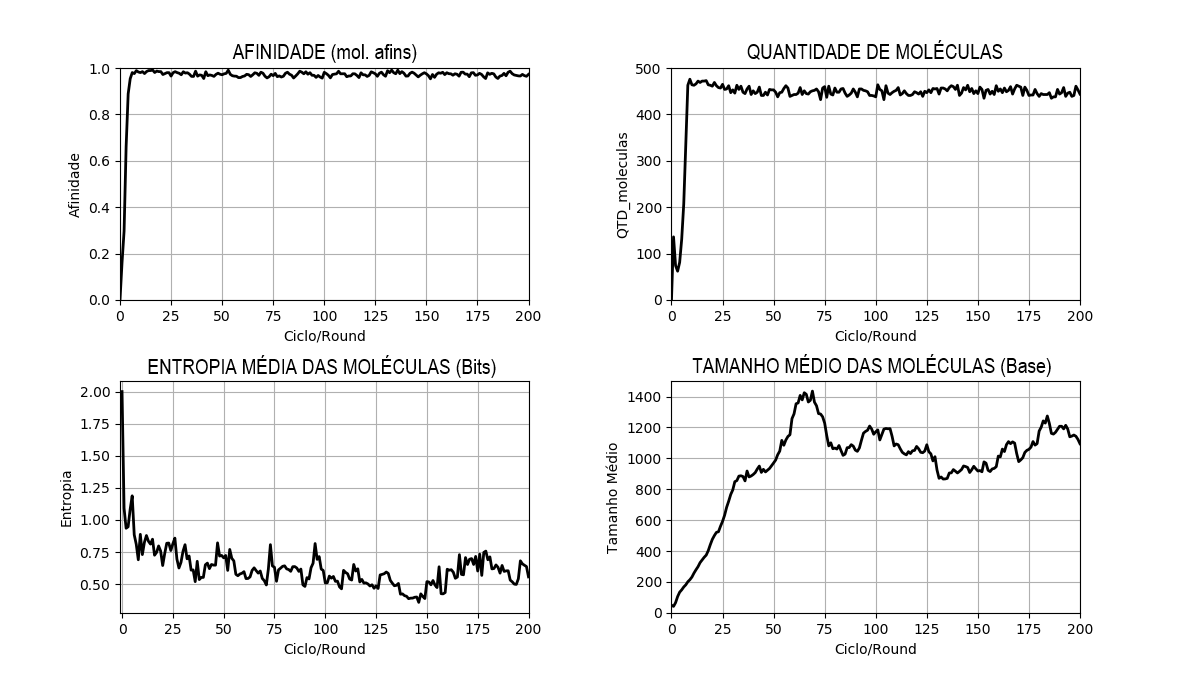
\includegraphics[width=15cm]{figures/image18_alpha05_beta_20.png}
    \caption{Cenário 2- Eficiência de filtro 20\%.}
    \label{fig:image18_alpha05_beta_20}
\end{figure}

\begin{figure}[!h]
    \centering
    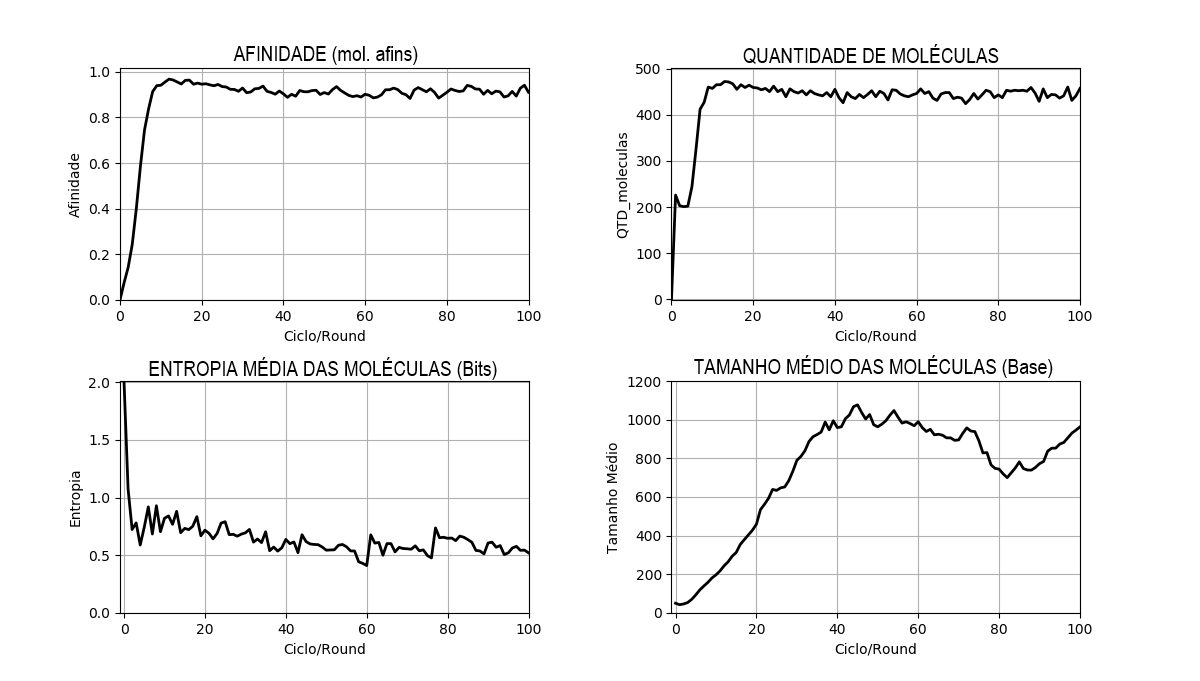
\includegraphics[width=15cm]{figures/image19_alpha05_beta_40.png}
    \caption{Cenário 2- Eficiência de filtro 40\%.}
    \label{fig:image19_alpha05_beta_40}
\end{figure}

\begin{figure}[!h]
    \centering
    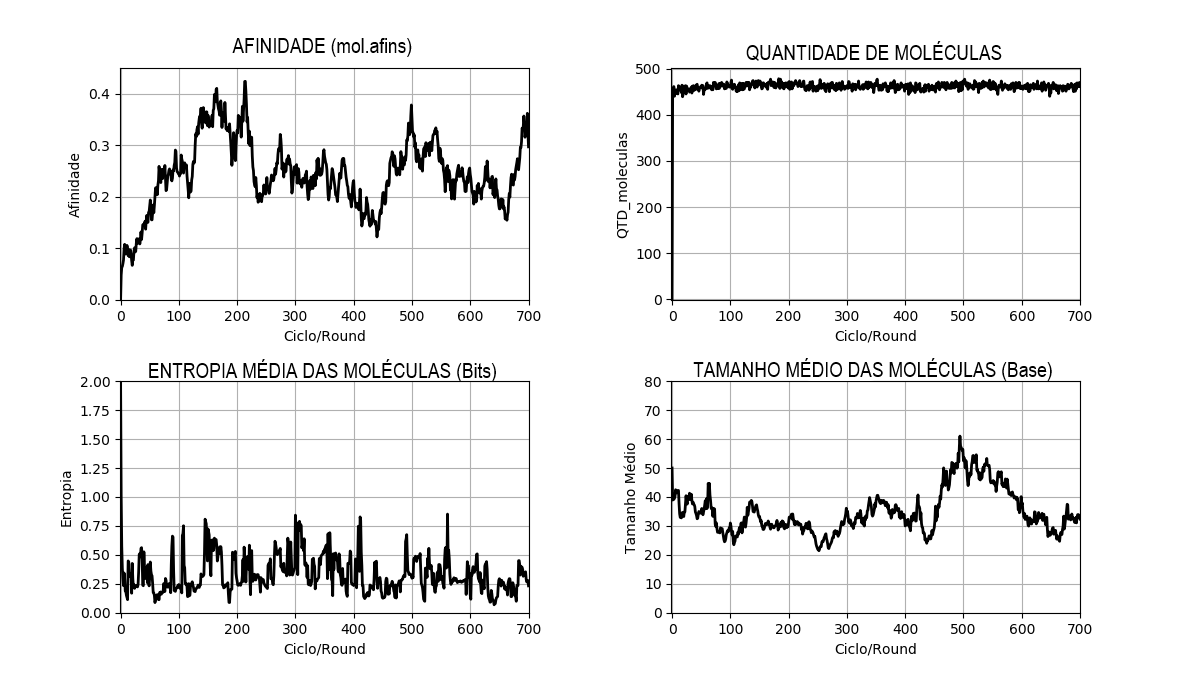
\includegraphics[width=15cm]{figures/image20_alpha05_beta_90.png}
    \caption{Cenário 2- Eficiência de filtro 90\%.}
    \label{fig:image20_alpha05_beta_90}
\end{figure}
\newpage

As figuras \ref{fig:image18_alpha05_beta_20}-\ref{fig:image20_alpha05_beta_90} sobre o cenário 2 mostram que o tamanho médio das moléculas
junto a quantidade de moléculas nunca se mostrava preciso a cada simulação e bem
instável ao decorrer dos ciclos, mostrando assim, que não foi escolhido o melhor método
para simulação.

\subsection{Cenário 3}

O último cenário foi bem mais complexo pois todas as moléculas que morrem
durante os ciclos são recolhidas as suas bases e colocadas no reservatório, onde, para
haver replicação de moléculas é necessário que tenha bases suficientes para a
replicação, caso não tenha a quantidade de bases necessária, a etapa é pulada o sistema
parte para a próxima. O sistema começa e termina com 50.000 moléculas na
simulação, ou seja, o valor fixo do cenário são os seguintes: tamanho inicial de 100
bases, 500 moléculas iniciais, 20\% eficiência de filtro (chance de uma moléculas nãoafim morrer), 0\% de chance de uma molécula afim morrer, 5\% de taxa de mutação,
500 moléculas de totais no round e o tamanho do filtro era de 5 bases onde a sequência
era escolhida aleatoriamente no início. Quanto aos valores de quebra e junção foram:
10\% de chance de uma molécula se quebrar caso encontre a sequência de 2 bases no
stop códon, para junção foram escolhidas as 5 bases complementares da sequência
escolhida pelo filtro para uma molécula ser apta (se a sequência afim fosse AATTG
seu complemento seria TTAAC) com 10\% de chance de junção.

\subsubsection{Variando a taxa de mutação}

\begin{figure}[!h]
    \centering
    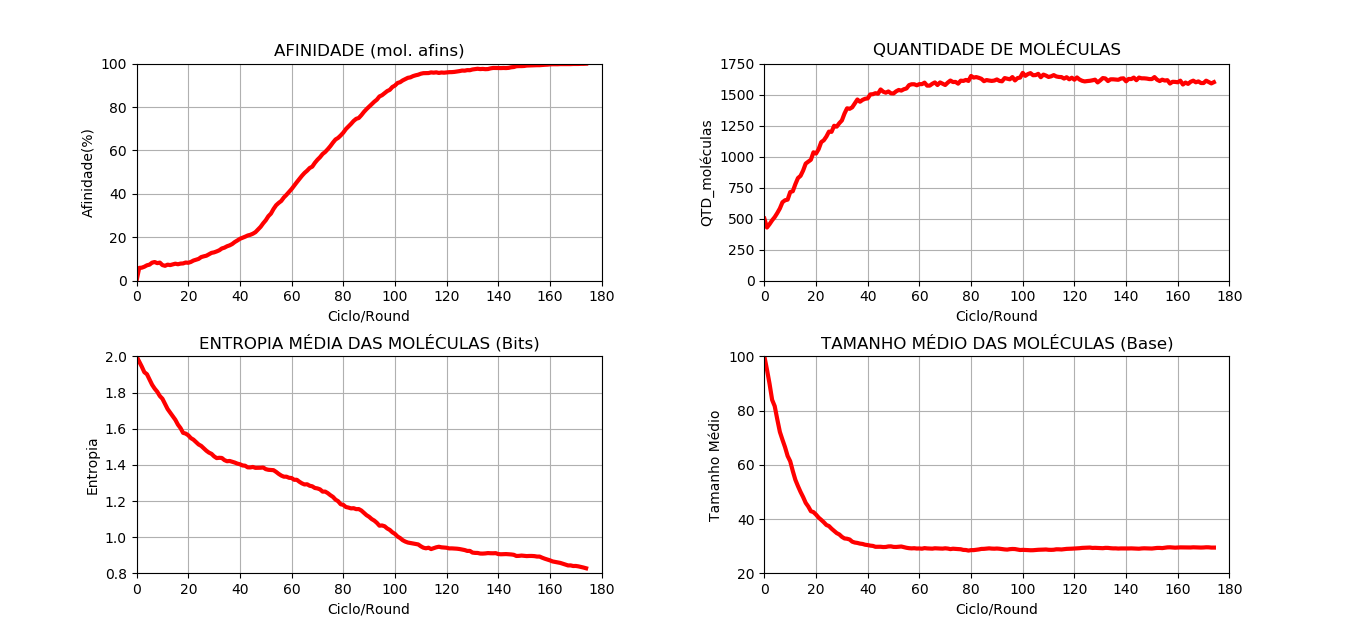
\includegraphics[width=15cm]{figures/image21_alpha01_beta_10.png}
    \caption{Cenário 3- Taxa de mutação 1\%.}
    \label{fig:image21_alpha01_beta_10}
\end{figure}

\begin{figure}[!h]
    \centering
    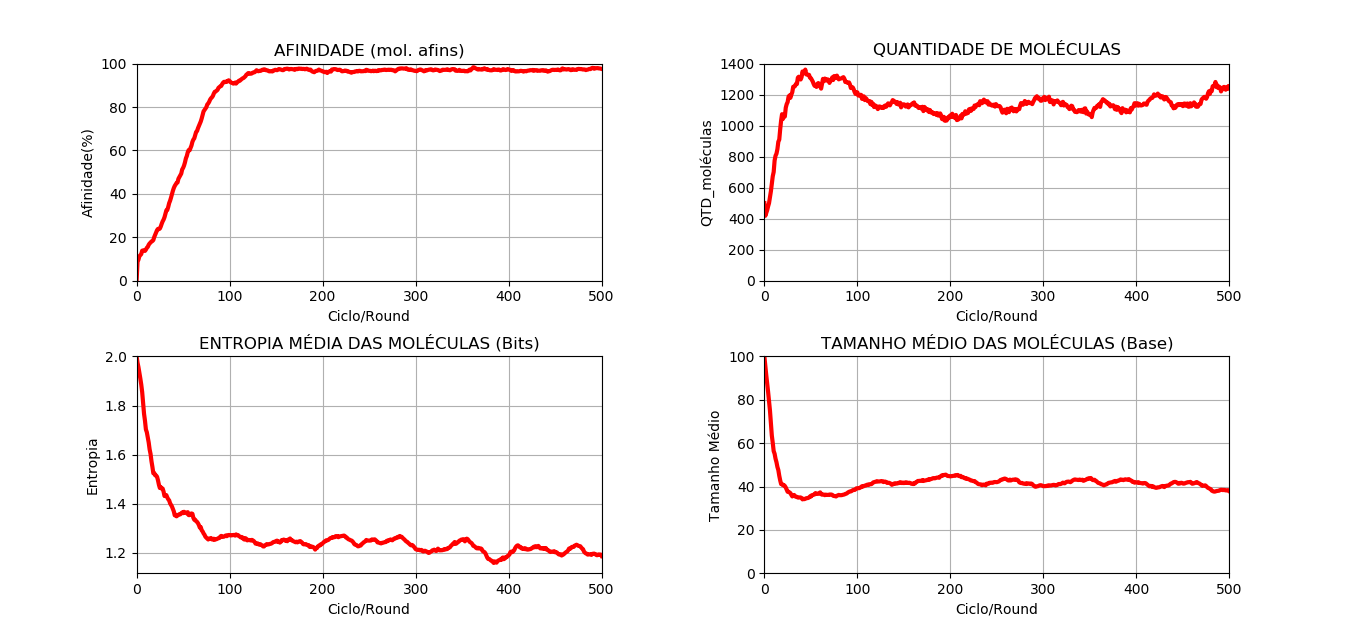
\includegraphics[width=15cm]{figures/image22_alpha02_beta_10.png}
    \caption{Cenário 3- Taxa de mutação 2\%.}
    \label{fig:image22_alpha02_beta_10}
\end{figure}

\begin{figure}[!h]
    \centering
    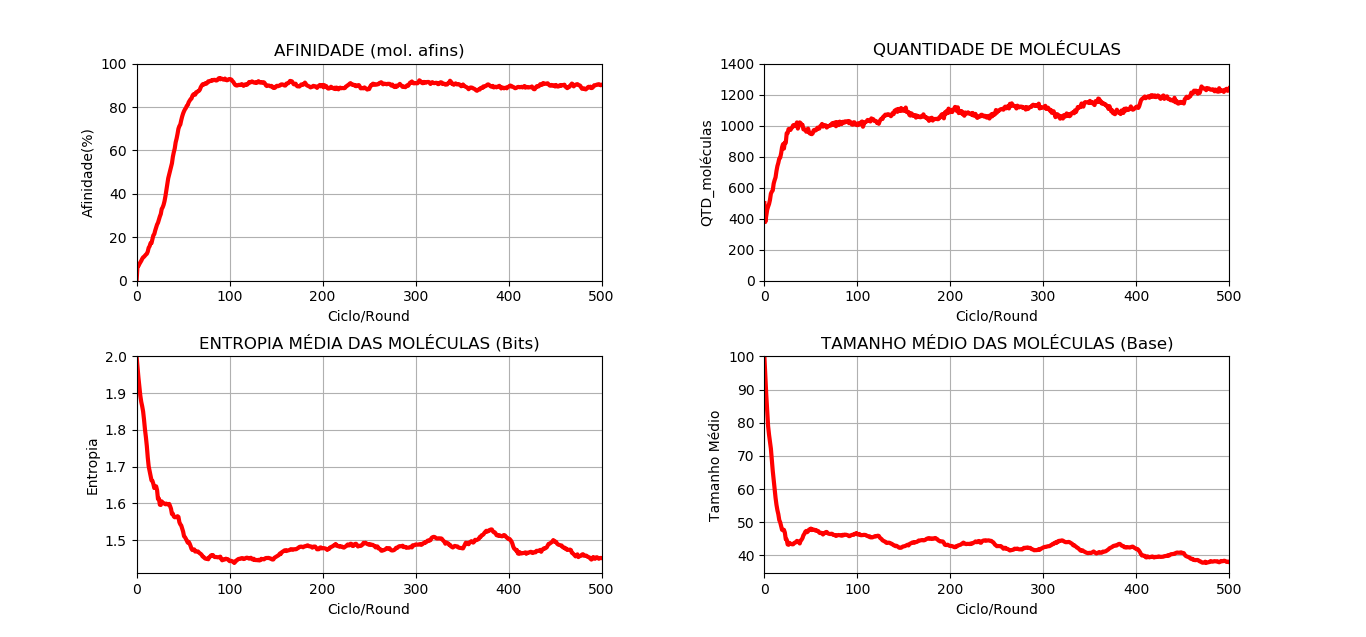
\includegraphics[width=15cm]{figures/image23_alpha05_beta_10.png}
    \caption{Cenário 3- Taxa de mutação 5\%.}
    \label{fig:image23_alpha05_beta_10}
\end{figure}

\begin{figure}[!h]
    \centering
    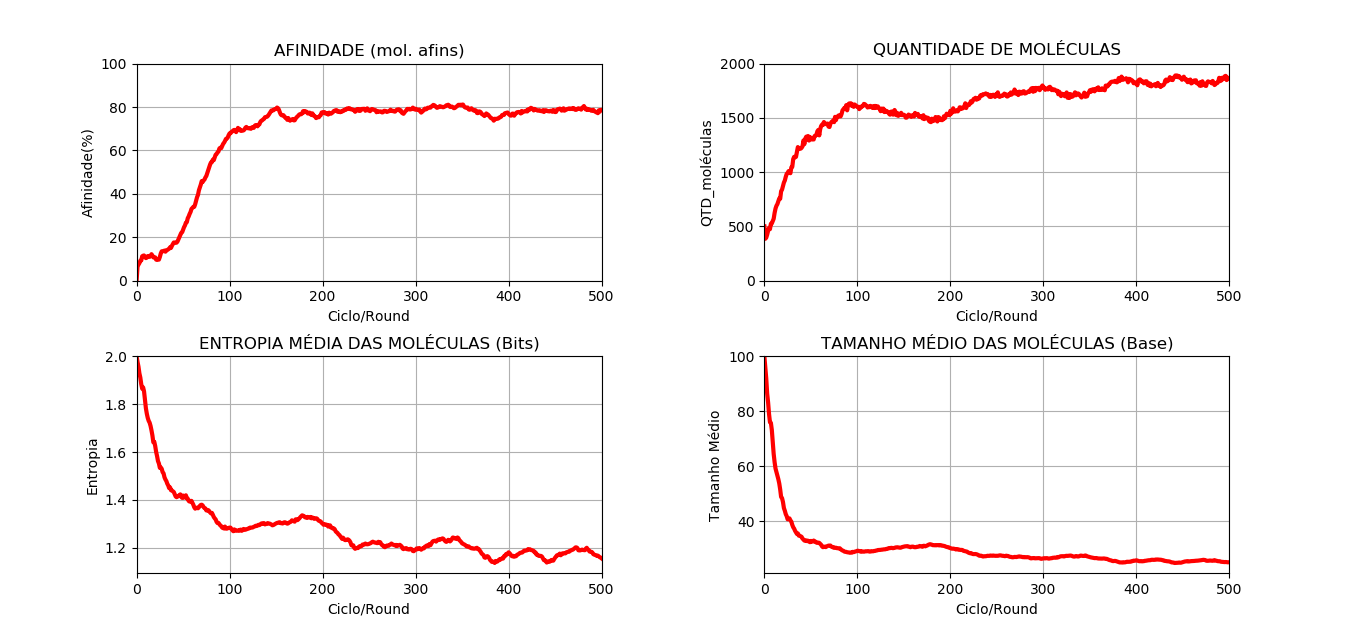
\includegraphics[width=15cm]{figures/image24_alpha10_beta_10.png}
    \caption{Cenário 3- Taxa de mutação 10\%.}
    \label{fig:image24_alpha10_beta_10}
\end{figure}

\newpage


Após análise das figuras \ref{fig:image21_alpha01_beta_10}-\ref{fig:image24_alpha10_beta_10} é perceptível foi um avanço na questão da quebra
e junção estarem bem mais suave no decorrer da simulação, porém podemos perceber
pelo tamanho das moléculas que cada vez mais iam diminuindo lentamente após a
instabilidade dos 100 primeiros ciclos, podemos tirar como conclusão 2 grandes
evidencias, sendo a primeira delas que mesmo a quebra e junção tenho 10% de
probabilidade de acontecer, o processo de quebra foi mais forte. A segunda é que, a
molécula ser pequena tendo no mínimo suficiente para estar no ciclo pode algo benéfico
pois estamos falando de uma molécula apta e pequena tornando-a forte e compacta.

